% APPENDIX
% State Space Intro
\chapter{Basics of State Space Modeling} \label{app.statespace}
\section{Introductory Concepts}

The differential equations of a lumped linear network can be written in the form
\begin{subequations}
\begin{flalign}
    \dot{\vec{x}}(t)    & = A\vec{x}(t) + B\vec{u}(t) \label{eq.stateeq}\\
    \vec{y}(t)    & = C\vec{x}(t) + D\vec{u}(t) \label{eq.outputeq}
\end{flalign}
\end{subequations}
Equation~(\ref{eq.stateeq}) is a system of first-order differential equations and is known as the \uline{state equation} of the system.  The vector $\vec{x}(t)$ is the \uline{state} vector, and $\vec{u}(t)$ is the \uline{input} vector.  Equation~(\ref{eq.outputeq}) is referred to as the \uline{output equation}.  $A$ is called the state matrix, $B$ the input matrix, $C$ the output matrix, and $D$ is the direct transition matrix.
\par
One advantage of the state space method is that the form lends itself easily to the digital and analog computation methods of solution.  Further, the state space method can be easily extended to the analysis of nonlinear systems.
\par
State equations may be obtained from an $n^{th}$ order differential equation or directly from the system model by identifying appropriate state variables.  To illustrate the first method, consider an $n^{th}$ order linear plant model described by the differential equation
\begin{equation}
    \frac{d^ny}{dt^n} + a_{n-1} \frac{d^{n-1}y}{dt^{n-1}} +
        \cdots + a_1 \frac{dy}{dt} + a_0 y = u(t)
        \label{eq.nthorder}
\end{equation}
Where $y(t)$ is the plant output and $u(t)$ is the plant input.  A state model for this system is not unique but depends on the choice of a set of state variables.  A useful set of state variables, referred to as \uline{phase variables}, is defined as:
\begin{equation}
    x_1 = y, \quad x_2 = \dot{y}, \quad x_3 = \ddot{y}, \ldots,
        x_n = \frac{d^{n-1}y}{dt^{n-1}}
        \label{eq.differentiatestate}
\end{equation}
\par
Taking derivatives of the first $n-1$ state variables, we have
\begin{equation}
    \dot{x}_1 = x_2, \quad \dot{x}_2 = x_3, \quad
        \ldots, \quad \dot{x}_{n-1} = x_n
    \label{eq.dotstatechain}
\end{equation}
In addition, $\dot{x}_n$ comes from rearranging Eq.~(\ref{eq.nthorder}) and substituting from Eq.~(\ref{eq.differentiatestate}):
\begin{equation}
    \dot{x}_n = -a_0x_1 - a_1x_2 -\cdots-a_{n-1}x_n + u(t)
    \label{eq.dotstatesub}
\end{equation}
In matrix form, this looks like
\begin{equation}
    \left[ \begin{array}{c} \dot{x}_1 \\ \dot{x}_2 \\ \vdots \\
                    \dot{x}_{n-1} \\ \dot{x}_n \end{array} \right]
    =
    \left[ \begin{array}{ccccc}
            0   &   1   &   0   &   \cdots  &   0   \\
            0   &   0   &   1   &   \cdots  &   0   \\
            \vdots&\vdots&\vdots&   \ddots  & \vdots\\
            0   &   0   &   0   &   \cdots  &   1   \\
            -a_0&   -a_1&   -a_2&   \cdots  &   -a_{n-1}
            \end{array} \right]
    \left[ \begin{array}{c} x_1 \\ x_2 \\ \vdots \\
                    x_{n-1} \\ x_n \end{array} \right]
    +
    \left[ \begin{array}{c} 0 \\ 0 \\ \vdots \\
                    0 \\ 1 \end{array} \right] u(t)
\end{equation}
Thus the output equation is simply
\begin{equation}
    y = \left[ \begin{array}{ccccc}1&0&0&\cdots&0\end{array} \right] \vec{x}
\end{equation}
\par
\begin{workex} \label{ex.phasevarstatespace}
Obtain the state equation in phase variable form for the following differential equation:
\begin{equation*}
    2\frac{d^3y}{dt^3} + 4\frac{d^2y}{dt^2} + 6\frac{dy}{dt} + 8y = 10u(t)
\end{equation*}
\textit{Solution}:
\par
The differential equation is third order, and thus there are three state variables: $x_1 = y$, $x_2 = \dot{y}$, and $x_3 = \ddot{y}$.  The first derivatives are:
\begin{flalign*}
    \dot{x}_1 & = x_2 \\
    \dot{x}_2 & = x_3 \\
    \dot{x}_3 & = -4x_1 - 3x_2 - 2x_3 + 5u(t)
\end{flalign*}
Or, in matrix form:
\begin{flalign*}
    \left[ \begin{array}{c} \dot{x}_1 \\ \dot{x}_2 \\ \dot{x}_3 \end{array}
        \right]
    & =
    \left[ \begin{array}{rrr}0&1&0\\0&0&1\\-4&-3&-2\end{array} \right]
    \left[ \begin{array}{c} x_1 \\ x_2 \\ x_3 \end{array} \right]
    +
    \left[ \begin{array}{c} 0\\0\\5 \end{array}\right] u(t)
    \\
    y & =
    \left[ \begin{array}{ccc}1&0&0\end{array}\right]
    \left[ \begin{array}{c} x_1 \\ x_2 \\ x_3 \end{array} \right]
\end{flalign*}
\end{workex}
\par
The m-file \verb=ode2phv.m= was developed to convert an $n^{th}$ order ordinary differential equation to the state space phase variable form.  The syntax is \verb#[A, B, C] = ode2phv(ai,k)#, and returns the typical three matrices.  The input \verb=ai= is a row vector containing the coefficients of the equation in descending order, and \verb=k= is the coefficient on the right hand side.  Using the ODE from Example \ref{ex.phasevarstatespace}, we would enter:

\begin{codex}
>> ai = [2 4 6 8];
>> k = 10;
>> [A, B, C] = ode2phv(ai,k)
A =
    0   1   0
    0   0   1
    -4  -3  -2
B =
    0
    0
    5
C =
    1   0   0
>>
\end{codex}

\subsubsection{Equations of Electrical Networks}
The state variables are directly related to the energy storage elements of a system.  It would seem, therefore, that the number of independent initial conditions is equal to the  number of energy storing elements.  This is true---provided that there is no loop containing only capacitors and voltage sources, and there is no cut set containing only inductive and current sources. In general, if there are $n_C$ loops of all capacitors and voltages sources, and $n_L$ cut sets of all inductors and current sources, the number of state variables is
\begin{equation}
    n = e_L + e_C - n_C - n_L
\end{equation}
where $e_L$ and $e_C$ are the numbers of inductors and capacitors, respectively.

\begin{figure}[bth]
\centering
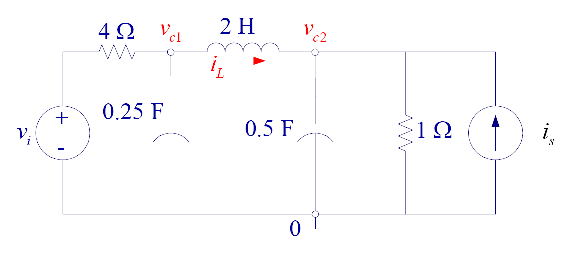
\includegraphics[width=.6\textwidth]{statespaceelecnet}
\caption{\footnotesize
        Circuit of Example~\ref{ex.elecnet}
        \label{fig.statespace.elecnet}
        }
\end{figure}

\begin{workex} \label{ex.elecnet}
Write the state equation for the network shown in Figure~\ref{fig.statespace.elecnet}.\\
\textit{Solution}:
\par
Define the state variables as current through the inductor and voltage across the capacitors.  Write two node equations containing capacitors and a loop equation containing the inductor.  The state variables will be $v_{c1}$, $v_{c2}$, and $i_L$.
\par
Node equations:
\begin{flalign*}
    0.25\frac{dv_{c1}}{dt} + i_L + \frac{v_{c1}-v_i}{4} = 0 & \Rightarrow
        \dot{v}_{c1} = -v_{c1} - 4i_L + v_i \\
    0.5 \frac{dv_{c2}}{dt} - i_L + v_{c2} - i_s = 0 & \Rightarrow
        \dot{v}_{c2} =  -2i_L +2 v_{c2} + 2i_s
\end{flalign*}
Loop equation:
\begin{flalign*}
    2\frac{di_L}{dt} + v_{c2} -v_{c1} = 0 & \Rightarrow
        \dot{i}_L = 0.5v_{c1} -0.5v_{c2}
\end{flalign*}
\par
Equivalently, in matrix form:
\begin{equation*}
    \left[ \begin{array}{c} \dot{v}_{c1} \\ \dot{v}_{c2} \\ \dot{i}_L
        \end{array} \right]
    =
    \left[ \begin{array}{rrr} -1&0&-4\\0&-2&2\\0.5&-0.5&0 \end{array}
        \right]
    \left[ \begin{array}{c} v_{c1} \\ v_{c2} \\ i_L
        \end{array} \right]
    +
    \left[ \begin{array}{cc} 1&0\\0&2\\0&0 \end{array}\right]
    \left[ \begin{array}{c} v_i \\ i_s \end{array} \right]
\end{equation*}
\end{workex}

\subsection{Simulation Diagrams}

Equations~(\ref{eq.dotstatechain}) and (\ref{eq.dotstatesub}) indicate that state variables are determined by integrating the corresponding state equation.  A diagram known as the \uline{simulation diagram} can be constructed to model the given differential equations.  The basic element of the simulation diagram is the integrator.  The first equation in (\ref{eq.dotstatechain}) is $\dot{x}_1  = x_2$.  Integrating we have:
\begin{equation*}
    x_1 = \int x_2 dx
\end{equation*}
\par
The above integral is represented by the time-domain block diagram shown in Figure~\ref{fig.statespace.inttimedom} and by the signal flow graph in Figure~\ref{fig.statespace.intsigflow}.

\newsavebox{\tempbig}
\newsavebox{\tempsmall}
\begin{figure}[bht]
\centering
\sbox{\tempbig}{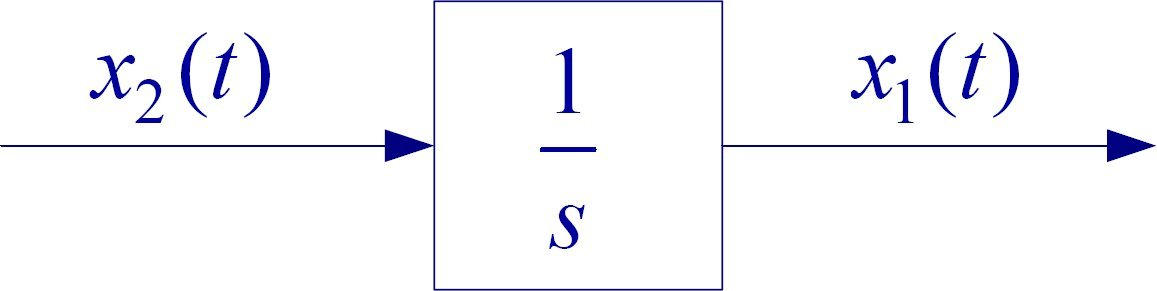
\includegraphics[width=.48\textwidth]{inttimedom}}
\sbox{\tempsmall}{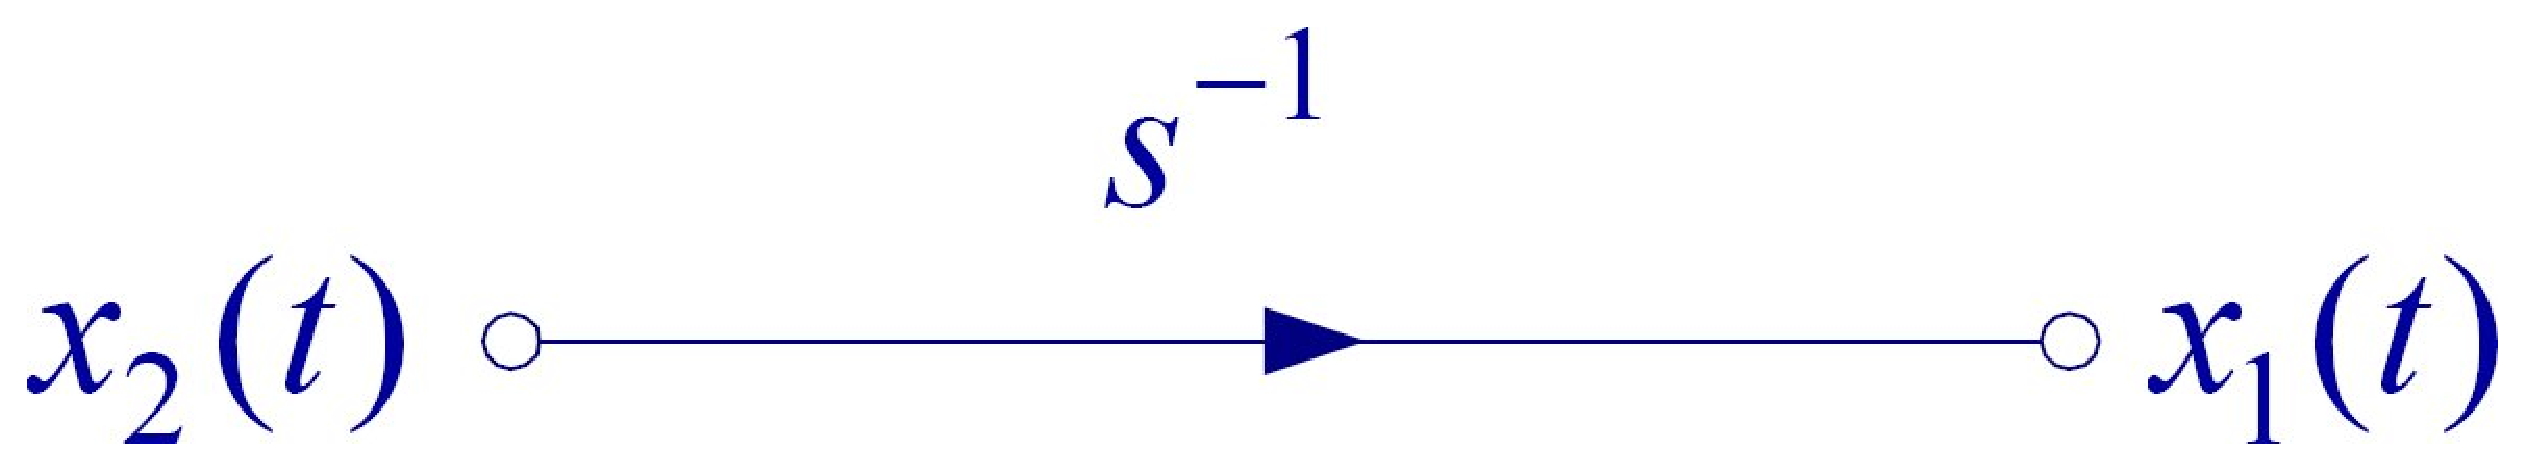
\includegraphics[width=.48\textwidth]{intsigflow}}
\newlength{\subfigoffset}
\setlength{\subfigoffset}{.5\ht\tempbig}
\addtolength{\subfigoffset}{-.5\ht\tempsmall}
\subfloat[Block diagram
            \label{fig.statespace.inttimedom}]{
            \usebox{\tempbig}
            }
\hfill
\subfloat[Signal flow graph
            \label{fig.statespace.intsigflow}]{
            \raisebox{\subfigoffset}{\usebox{\tempsmall}}
            }
\caption{\footnotesize
        Simulation diagrams: Graphical representations of state integrators in the time domain.
        \label{fig.statespace.integratorgraphs}
        }
\end{figure}
\par

It is important to know that that although the symbol $\frac{1}{s}$ is used for integration, the simulation diagram is still a time-domain representation.  The number of integrators is equal to the number of state variables.  For example, for the state equation in Example~\ref{ex.phasevarstatespace} we have three integrators in cascade, the three state variables are assigned to the output of each integrator as shown in Figure~\ref{fig.statespace.phasevardiagram}.  The final state equation---seen in (\ref{eq.dotstatesub})---is represented via a summing point and feedback paths.  Completing the output equation, we obtain the simulation diagram known as \uline{phase-variable control canonical form} (See Fig.\ \ref{fig.statespace.phasevardiagramsigflow}).

\begin{figure}[bht]
\centering
\sbox{\tempbig}{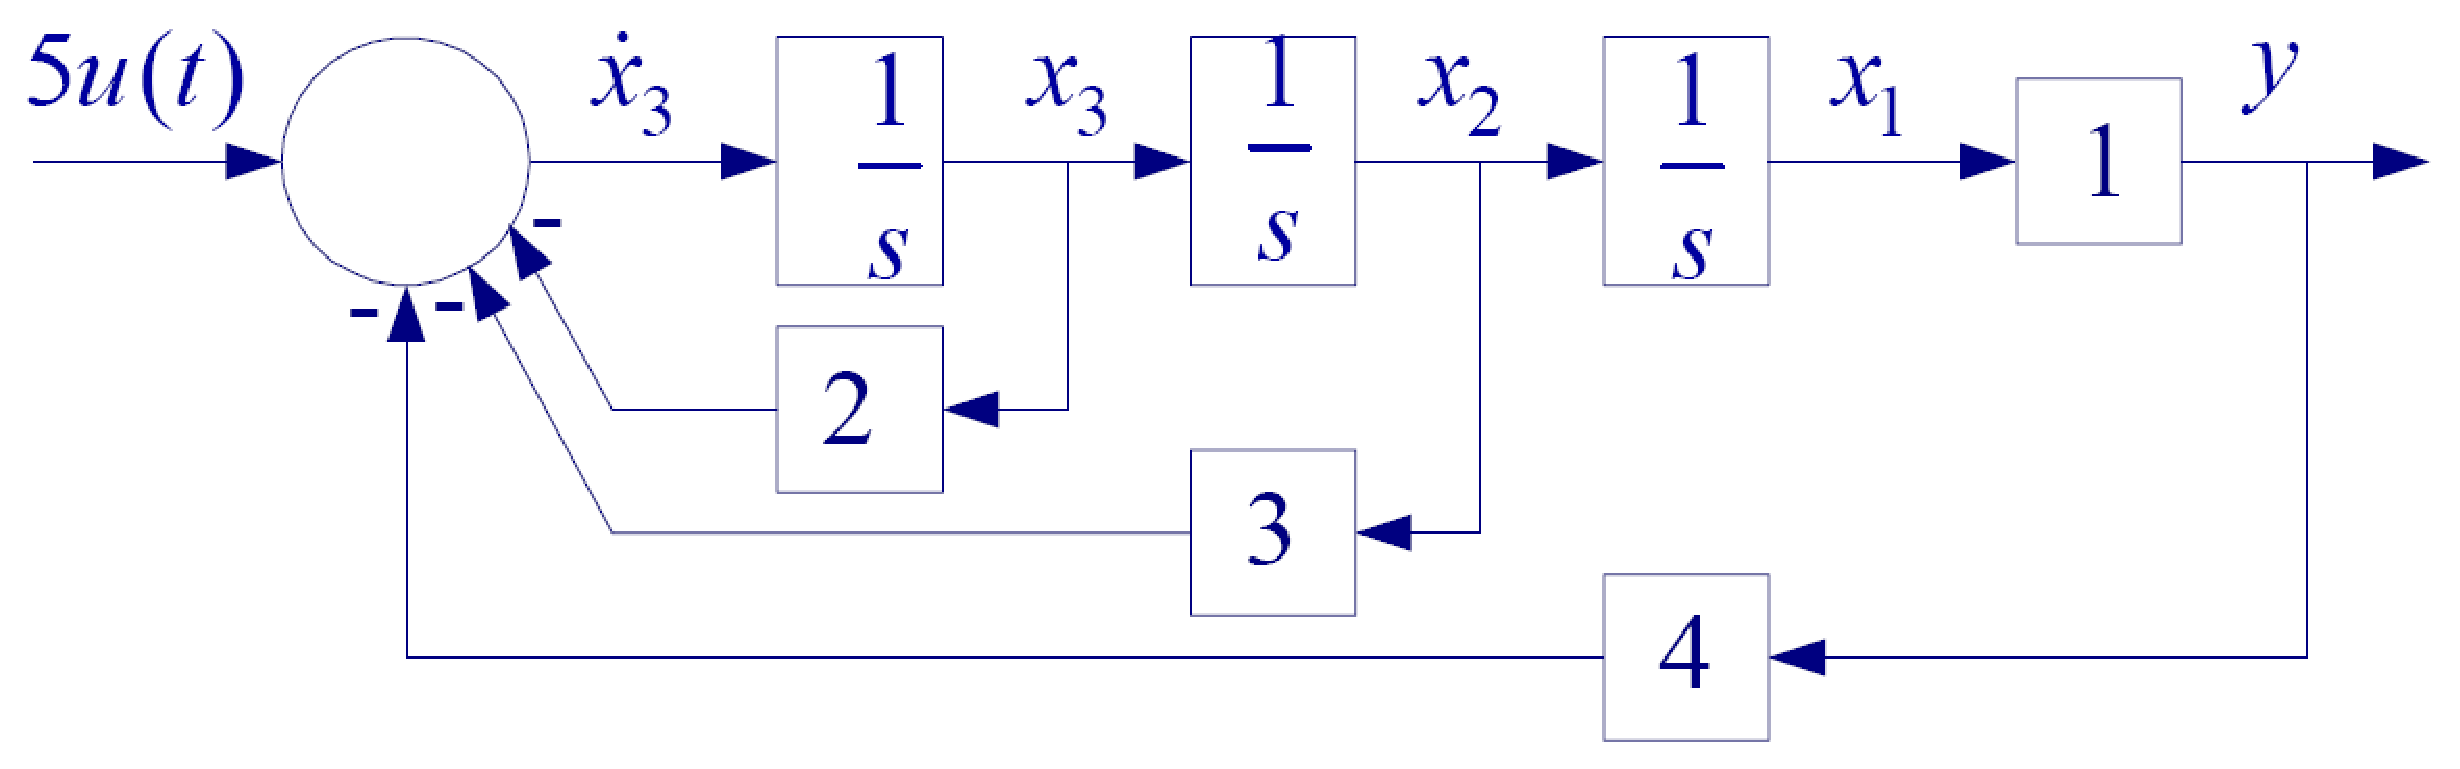
\includegraphics[width=.45\textwidth]{phasevarblock}}
\sbox{\tempsmall}{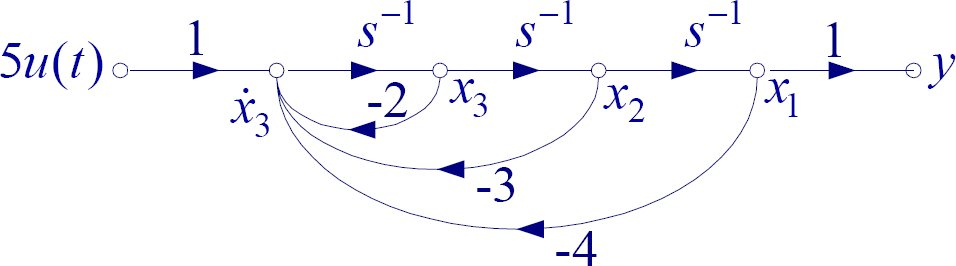
\includegraphics[width=.45\textwidth]{phasevarsigflow}}
\newlength{\subfigoffsetB}
\setlength{\subfigoffsetB}{.5\ht\tempbig}
\addtolength{\subfigoffsetB}{-.5\ht\tempsmall}
\subfloat[Block diagram]{
            \usebox{\tempbig}
            }
\hfill
\subfloat[Signal flow]{\label{fig.statespace.phasevardiagramsigflow}
            \raisebox{\subfigoffsetB}{\usebox{\tempsmall}}
            }
\caption{\footnotesize
        Simulation diagrams for Example~\ref{ex.phasevarstatespace} in phase-variable control canonical form.
        \label{fig.statespace.phasevardiagram}
        }
\end{figure}

\subsection{Transfer Function to State Space Conversion}

Consider the transfer function of a third-order system where the numerator degree is lower than that of the denominator.
\begin{equation}
    \frac{Y(s)}{U(s)} = \frac{b_2 s^2 + b_1 s + b_0}{
        s^3 + a_2 s^2 + a_1 s + a_0}
    \label{eq.thirdorderTF}
\end{equation}
The above transfer function is decomposed into two (frequency domain) blocks in Figure~\ref{fig.statespace.TFblockdecomp}.

\begin{figure}[bht]
\centering
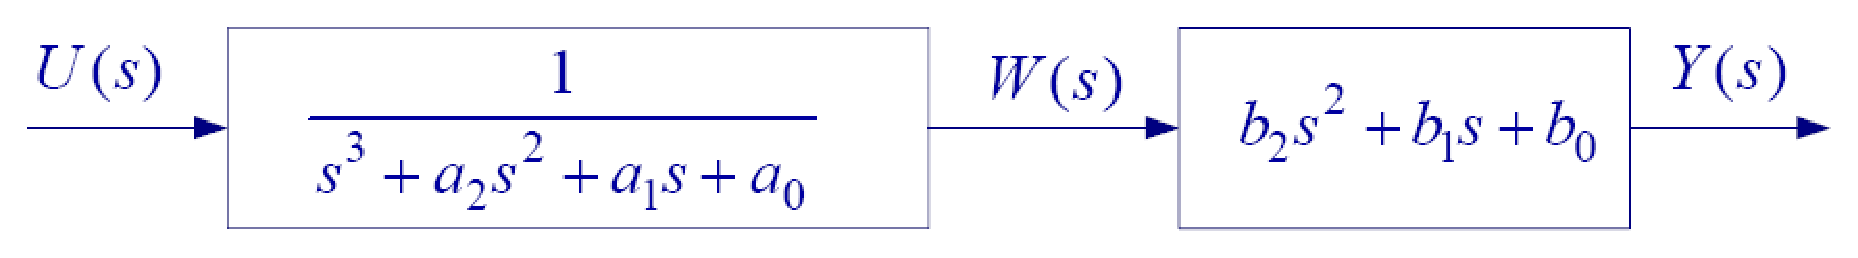
\includegraphics[width=0.8\textwidth]{TFblockdecomp}
\caption{\footnotesize
        The transfer function of Eq.\ (\ref{eq.thirdorderTF}) arranged in cascade form
        \label{fig.statespace.TFblockdecomp}
        }
\end{figure}

Denoting the output of the first block as $W(s)$, we have the following input/output relationships:
\begin{subequations}
\begin{gather}
    W(s) = \frac{U(s)}{s^3 + a_2 s^2 + a_1 s + a_0}
        \label{eq.inputstate} \\
    Y(s) = b_2 s^2 W(s) + b_1 s W(s) + b_0 W(s)
        \label{eq.outputstate}
\end{gather}
\end{subequations}
Rearranging Eq.\ (\ref{eq.inputstate}), we get
\begin{equation}
    s^3 W(s) = -a_2 s^2 W(s) - a_1 s W(s) - a_0 W(s) + U(s)
    \label{eq.inputstaterearrange}
\end{equation}
Using properties of frequency-domain tranforms, we see that Equations~(\ref{eq.inputstaterearrange}) and (\ref{eq.outputstate}) are the frequency-domain representations of the following time-domain differential equations:
\begin{subequations}
\begin{gather}
    \dddot{w} = -a_2 \ddot{w} - a_1 \dot{w} - a_0 w + u(t) \\
    y(t) = b_2 \ddot{w} + b_1 \dot{w} + b_0 w
\end{gather}
\end{subequations}

From the above expressions, we see that $\dddot{w}$ has to go through three integrators to get $w$ (as shown in Figure~\ref{fig.statespace.tripleintblock}).  Completing the above equations results in the phase-variable control canonical simulation diagram.

\begin{figure}[hbt]
\centering
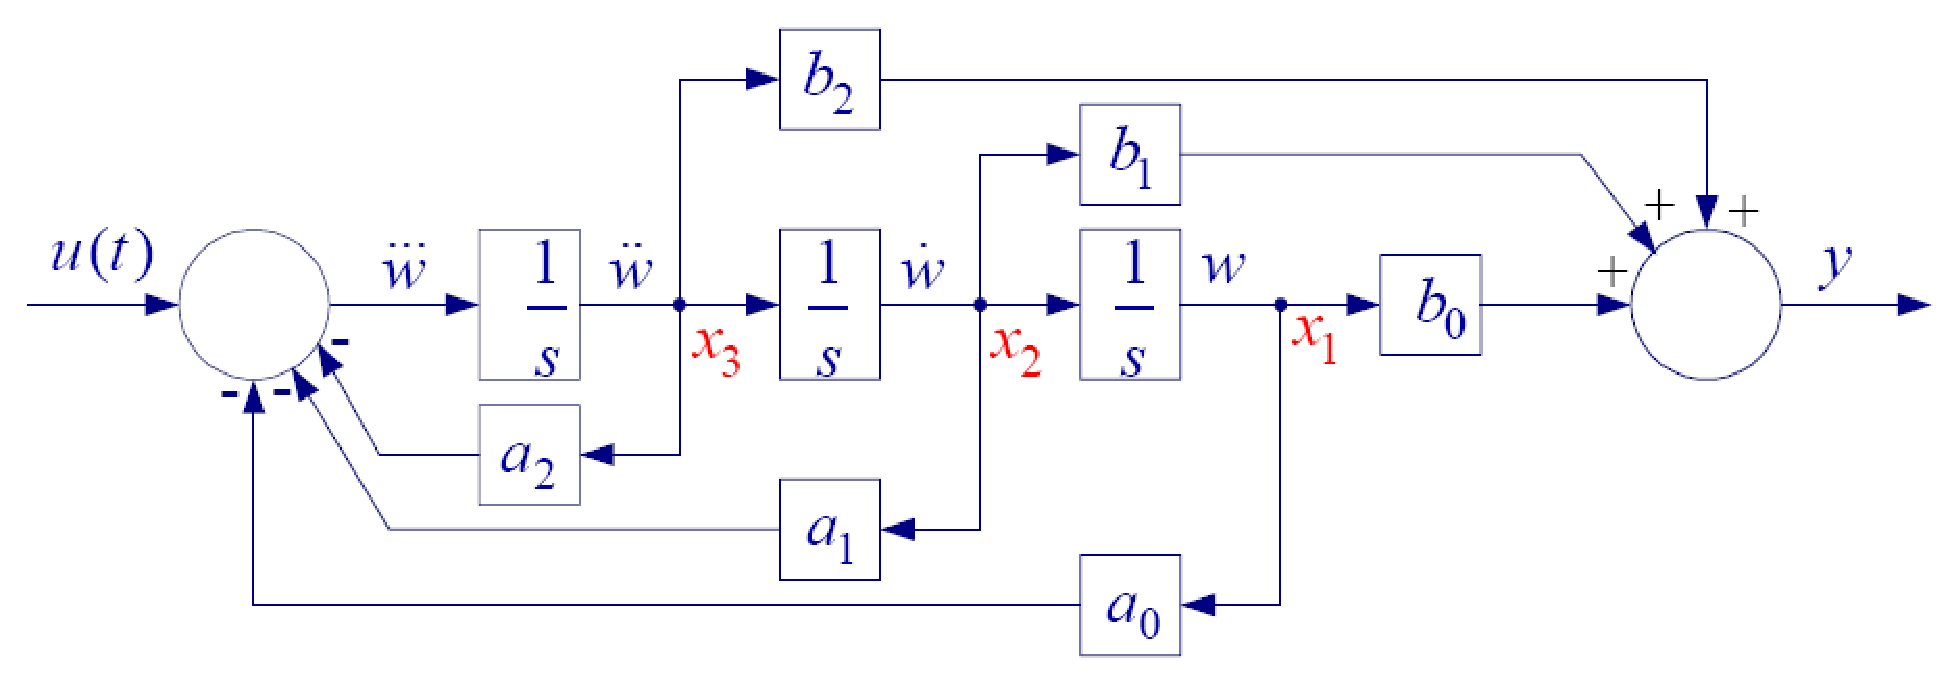
\includegraphics[width=.9\textwidth]{tripleintblock}
\caption{\footnotesize
        Phase variable control canonical simulation block diagram for the transfer function in Eq.~(\ref{eq.thirdorderTF})
        \label{fig.statespace.tripleintblock}
        }
\end{figure}

Figure~\ref{fig.statespace.tripleintblock} is a block diagram suitable for Simulink analysis.  You may find it easier to construct the simulation diagram similar to the signal flow graph as shown in Figure~\ref{fig.statespace.tripleintsigflow}.

\begin{figure}[thb]
\centering
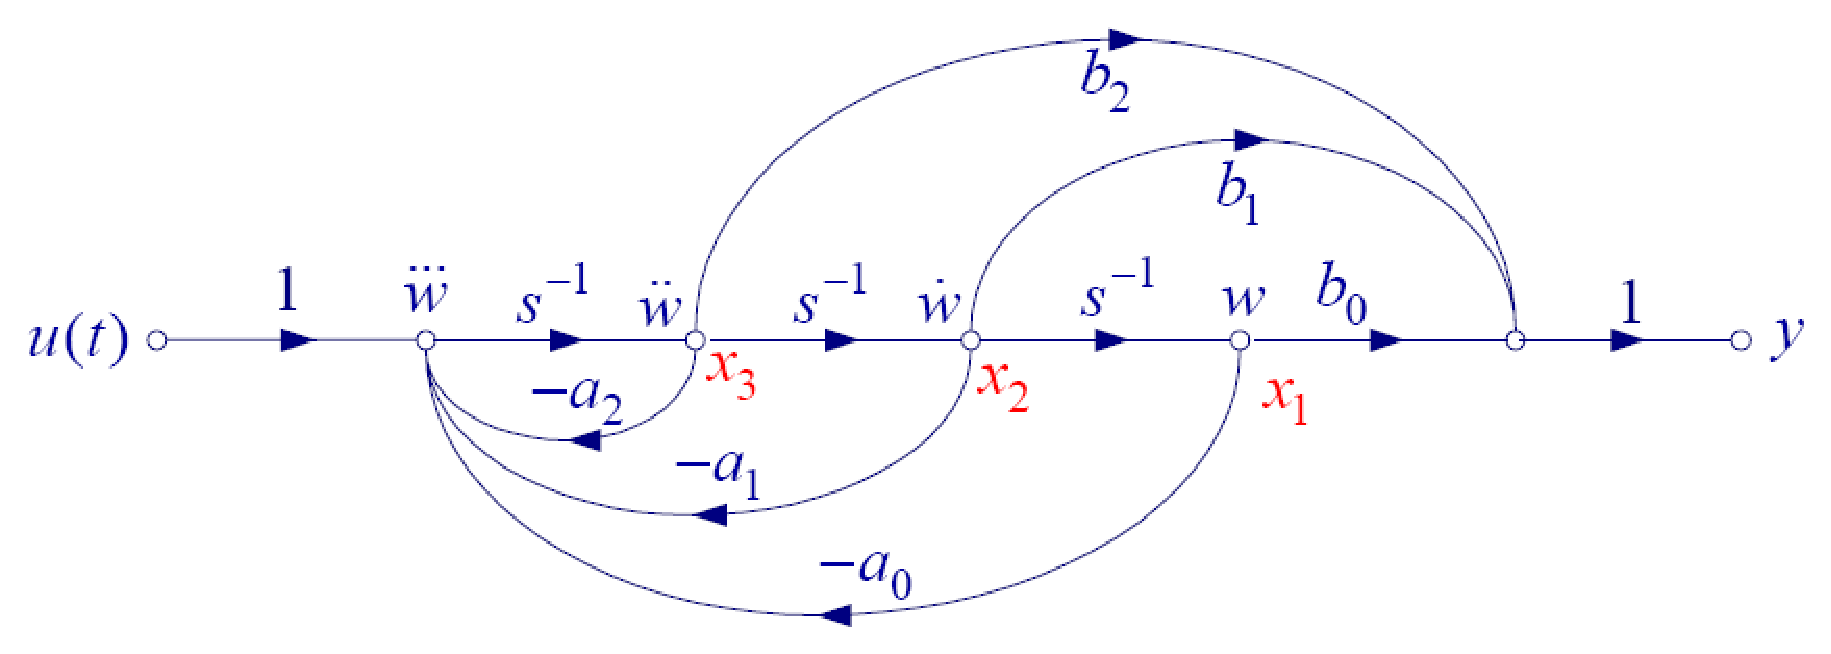
\includegraphics[width=0.9\textwidth]{tripleintsigflow}
\caption{\footnotesize
        Phase variable control canonical signal flow diagram for the transfer function in Eq.~(\ref{eq.thirdorderTF})
        \label{fig.statespace.tripleintsigflow}
        }
\end{figure}

In order to write the state equation, the state variables $x_1(t)$, $x_2(t)$, and $x_3(t)$ are assigned to the output of each integrator from right to left in Figs.\ \ref{fig.statespace.tripleintblock} and \ref{fig.statespace.tripleintsigflow}.  Next, an equation is written for the input of each integrator:
\begin{flalign*}
    \dot{x}_1 & = x_2 \\
    \dot{x}_2 & = x_3 \\
    \dot{x}_3 & = -a_0 x_1 -a_1 x_2 - a_2 x_3 + u(t)
\end{flalign*}
and the output equation is $y = b_0 x_1 + b_1 x_2 + b_2 x_3$.  Once again, lumping it into matrix form, we get
\begin{equation}
\begin{split}
    \left[ \begin{array}{c} \dot{x}_1 \\ \dot{x}_2 \\ \dot{x}_3
            \end{array} \right]
    & =
    \left[ \begin{array}{ccc} 0&1&0\\0&0&1\\-a_0&-a_1&-a_2
            \end{array} \right]
    \left[ \begin{array}{c} x_1 \\ x_2 \\ x_3
            \end{array} \right]
    +
    \left[ \begin{array}{c} 0 \\ 0 \\ 1
            \end{array} \right]
    u(t)
    \\
    y & =
    \left[ \begin{array}{ccc} b_0&b_1&b_2 \end{array} \right]
    \left[ \begin{array}{c} x_1 \\ x_2 \\ x_3
            \end{array} \right]
    \label{eq.tripleintstatespace}
\end{split}
\end{equation}

It is important to note that Mason's gain formula can be applied to the simulation diagram in Fig.\ \ref{fig.statespace.tripleintsigflow} to obtain the original transfer function.  Indeed, the determinant of the matrix $sI-A$ from Eq.~(\ref{eq.tripleintstatespace}) yields the characteristic equation (often denoted $\Delta$) for Mason's rule.  See Section 2.7 of \cite{dorf} for more on Mason's rule.
\par
In conclusion, it is important to remember that there is no unique state space representation for a given transfer function.  The state space often depends on the application involved, the complexity of the model, and the individual engineer!
\par
The Control System Toolbox in MATLAB contains a set of functions for model conversion.  Specifically, \verb#[A, B, C, D] = tf2ss(num,den)# converts the transfer function fraction to state space phase-variable control canonical form.

\pagebreak[4]
 %\setlength{\hsize}{.9\textwidth}
\begin{workex} \label{ex.TFtoSS}
\begin{equation*}
    G(s) = \frac{Y(s)}{U(s)} =
        \frac{s^2 + 7s + 2}{s^3 + 9s^2 + 26s + 24}
\end{equation*}

For the above transfer function, do the following:
\begin{enumerate}
    \item Draw the simulation diagram and find a state space representation.
    \item Use the MATLAB Control System Toolbox function \texttt{tf2ss} to find a state model.
\end{enumerate}
\textit{Solution}:
\par
1. The transfer function in block diagram cascade form looks like Figure~\ref{fig.ex.statespace.TFblock}.
\par
From this we have
\begin{flalign*}
    s^3W(s) &= -9Ws^2W(s) - 26sW(s) - 24W(s) + U(s) \\
    Y(s)    &= s^2W(s) + 7sW(s) +2W(s)
\end{flalign*}
Converting these to the time domain:
\begin{flalign*}
    \dddot{w}   &= -9\ddot{w} - 26\dot{w} - 24w + u \\
    y(t)        &= \ddot{w} + 7\dot{w} + 2w
\end{flalign*}
The time-domain equations above yield the simulation diagram in Figure~\ref{fig.ex.statespace.TFsigflow}.
\par
To obtain the state equation, the state variables $x_1(t)$, $x_2(t)$, and $x_3(t)$ are assigned to the output of each integrator from right to left.  The equations corresponding to the input of each integrator are:
\begin{flalign*}
    \dot{x}_1 & = x_2 \\
    \dot{x}_2 & = x_3 \\
    \dot{x}_3 & = -24x_1 - 26x_2 - 9x_3 + u(t)
\end{flalign*}
The output equation is the summation of the feedforward links: $y = 2x_1 + 7x_2 +x_3$.
\par
Finally, in matrix form we have
\begin{flalign*}
    \left[ \begin{array}{c} \dot{x}_1 \\ \dot{x}_2 \\ \dot{x}_3
            \end{array} \right]
    & =
    \left[ \begin{array}{ccc} 0&1&0\\0&0&1\\-24&-26&-9
            \end{array} \right]
    \left[ \begin{array}{c} x_1 \\ x_2 \\ x_3
            \end{array} \right]
    +
    \left[ \begin{array}{c} 0 \\ 0 \\ 1
            \end{array} \right]
    u(t)
    \\
    y & =
    \left[ \begin{array}{ccc} 2&7&1 \end{array} \right]
    \left[ \begin{array}{c} x_1 \\ x_2 \\ x_3
            \end{array} \right]
\end{flalign*}
2. We write the following statements to check our results in MATLAB:
\begin{verbatim}
>> num = [1 7 2]; den = [1 9 26 24];
>> [A, B, C, D] = tf2ss(num,den)
A =                 B =         C =             D =
    -9  -26 -24         1           1   7   2       0
    1   0   0           0
    0   1   0           0
>>
\end{verbatim}
\end{workex}
\par
It is important to realize that parts 1 and 2 of Example~\ref{ex.TFtoSS} are equivalent.  MATLAB simply numbers the state variables in a different order.  To confirm this, we need only perform a simple substitution for one set of state variables.

\begin{figure}[bht]
\centering
\subfloat[Block diagram of the transfer function in cascade
        \label{fig.ex.statespace.TFblock}]{
        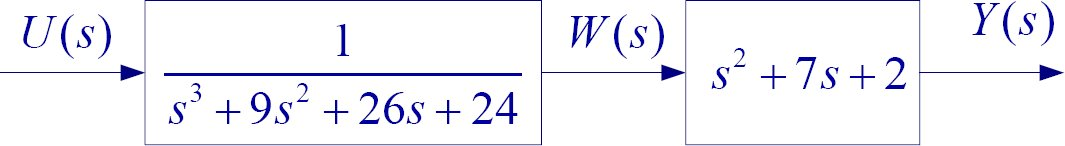
\includegraphics[width=0.7\textwidth]{TFtoSSblock}
        }
\newline
\subfloat[Signal flow simulation digram
        \label{fig.ex.statespace.TFsigflow}]{
        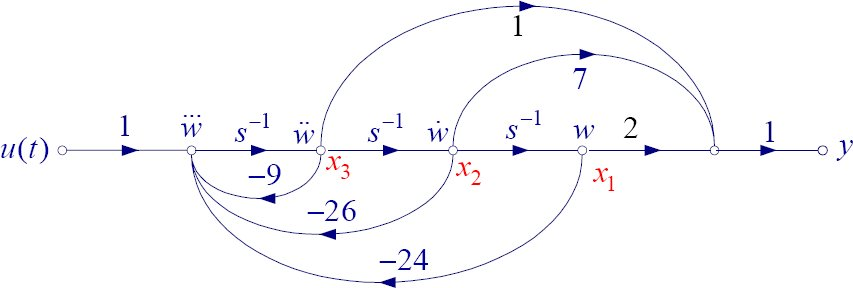
\includegraphics[width=0.8\textwidth]{TFtoSSsigflow}
        }
\caption{\footnotesize
        Diagrams for Example~\ref{ex.TFtoSS}
        }
\end{figure}

\subsection{State Space to Transfer Function Conversion}
Consider the state equation (\ref{eq.stateeq}).  We may take its Laplace transform and rearrange it as follows:
\begin{equation*}
    sX(s) = AX(s) + BU(s) \Rightarrow (sI - A)X(s) = BU(s)
\end{equation*}
If we combine this with the transform of the output equation: $Y(s) = CX(s) + DU(s)$, we get
\begin{equation*}
    Y(s) = C(sI - A)^{-1} BU(s) + DU(s)
\end{equation*}
or, equivalently
\begin{equation}
    \frac{Y(s)}{U(s)} = C(sI-A)^{-1} B+D
    \label{eq.TFfromSS}
\end{equation}
\par
In the Control Systems Toolbox, the command \verb#[num, den] = ss2tf(A,B,C,D,i)# converts the state equation to a transfer function for the $i^{th}$ input.

\begin{workex} \label{ex.SStoTF}
\begin{flalign*}
    \left[ \begin{array}{c} \dot{x}_1 \\ \dot{x}_2
            \end{array} \right]
    & =
    \left[ \begin{array}{cc} 0&1\\-6&-5
            \end{array} \right]
    \left[ \begin{array}{c} x_1 \\ x_2
            \end{array} \right]
    +
    \left[ \begin{array}{c} 0  \\ 1
            \end{array} \right]
    u(t)
    \\
    y & =
    \left[ \begin{array}{cc} 8&1 \end{array} \right]
    \left[ \begin{array}{c} x_1 \\ x_2
            \end{array} \right]
\end{flalign*}
Obtain the transfer function for the system described in the above state space model.\\
\textit{Solution}:
\par
Use the formula in Eq.\ (\ref{eq.TFfromSS}).
\begin{flalign*}
    sI - A &= \left[ \begin{array}{cc} s & -1 \\ 6 & s+5
                        \end{array} \right] \\
    \Rightarrow \Phi(s) := (sI - A)^{-1} &=
        \frac{\left[ \begin{array}{cc} s+5 & 1 \\ -6 & s
                        \end{array} \right]}{s^2+5s+6} \\
    \Rightarrow G(s) := C(sI-A)^{-1}B &=
        \left[ \begin{array}{cc} 8&1 \end{array} \right]
        \frac{\left[ \begin{array}{cc} s+5 & 1 \\ -6 & s
                        \end{array} \right]
                        \left[ \begin{array}{c}0\\1\end{array}\right]}
                        {s^2+5s+6} \\
    &= \frac{\left[ \begin{array}{cc} 8&1 \end{array} \right]
                \left[ \begin{array}{c}1\\s\end{array}\right]}
            {s^2+5s+6}
\end{flalign*}
Therefore the transfer function is
\begin{equation*}
    G(s) = \frac{s+8}{s^2+5s+6}
\end{equation*}
\end{workex}

\begin{workex} \label{ex.SStoTFmatlab}
\begin{flalign*}
    \left[ \begin{array}{c} \dot{x}_1 \\ \dot{x}_2 \\ \dot{x}_3
            \end{array} \right]
    & =
    \left[ \begin{array}{ccc} 0&1&0\\0&0&1\\-1&-2&-3
            \end{array} \right]
    \left[ \begin{array}{c} x_1 \\ x_2 \\ x_3
            \end{array} \right]
    +
    \left[ \begin{array}{c} 10 \\ 0 \\ 0
            \end{array} \right]
    u(t)
    \\
    y & =
    \left[ \begin{array}{ccc} 1&0&0 \end{array} \right]
    \left[ \begin{array}{c} x_1 \\ x_2 \\ x_3
            \end{array} \right]
\end{flalign*}
Use MATLAB to find the transfer function corresponding to the above state space model.\\
\textit{Solution}:
\begin{verbatim}
>> A = [0 1 0; 0 0 1; -1 -2 -3]; B = [10; 0; 0];
>> C = [1 0 0]; D = [0];
>> [num, den] = ss2tf(A,B,C,D,1);
>> G = tf(num,den)
G =
    10 s^2 + 30 s + 20
   ---------------------
   s^3 + 3 s^2 + 2 s + 1
>>
\end{verbatim}
\end{workex}

Also, \verb#[z, p, k] = ss2zp(A,B,C,D,i)# converts the state equations to the transfer function in factored form.
\par
MATLAB's Control System Toolbox contains many functions for model creation and inversion, data extraction, and system interconnections.  A few of these functions for continuous-time control systems are listed in Table~\ref{tab.statespace.ConSysTool}.  For a complete list of the toolbox's functions, type \verb=help/control/control= at the command prompt.

\begin{table}[bht]
\centering
\begin{tabular}{c|p{0.6\textwidth}}
    \textit{Command}& \multicolumn{1}{c}{\textit{Description}}\\ \hline \hline
    \verb=tf=       &   Create transfer function models \\
    \verb=zpk=      &   Create zero/pole/gain models \\
    \verb=ss=       &   Create state space models \\
    \verb=tfdata=   &   Extract numerators and denominators \\
    \verb=zpkdata=  &   Extract zero/pole/gain data \\
    \verb=ssdata=   &   Extract state space matrices \\
    \verb=append=   &   Group LTI systems by appending inputs and outputs \\
    \verb=parallel= &   Generalized parallel connection \\
    \verb=series=   &   Generalized series connection \\
    \verb=feedback= &   Feedback connection of two systems \\
    \verb=connect=  &   Derive state space model from block diagram description \\
    \verb=blkbuild= &   Builds a model from a block diagram
\end{tabular}
\caption{\footnotesize
        Important continuous-time control system commands
        \label{tab.statespace.ConSysTool}
        }
\end{table}

The Control System Toolbox supports three commonly used representations of linear time-invariant (LTI) systems: \verb=tf=, \verb=zpk=, and \verb=ss= objects.  To create an LTI model or object, use the corresponding constructor. For example, \verb#sys = tf(1,[1 0])# creates the transfer function $H(s) = 1/s$.  The resulting variable \verb=sys= is a \verb=tf= object containing the numerator and denominator data.  You can now treat the entire model as a single MATLAB variable.  For more details and examples on how to specify the various types of LTI models, type \verb=ltimodels= followed by the construct type at the MATLAB command prompt.
\par
The functions \verb=tfdata=, \verb=zpkdate=, and \verb=ssdata= are provided for extracting the parameters of their corresponding objects.  For example, the command \verb#[num, den] = tfdata(T,'v')# returns the numerator and denominator of the \verb=tf= object \verb=T=.  The argument \verb='v'= formats the outputs as row vectors rather than cell arrays.
\par
The Control System Toolbox contains many more commands that allow the construction of a system out of its components.  The lower entries in Table~\ref{tab.statespace.ConSysTool} are useful for this purpose.

\begin{figure}[thb]
\centering
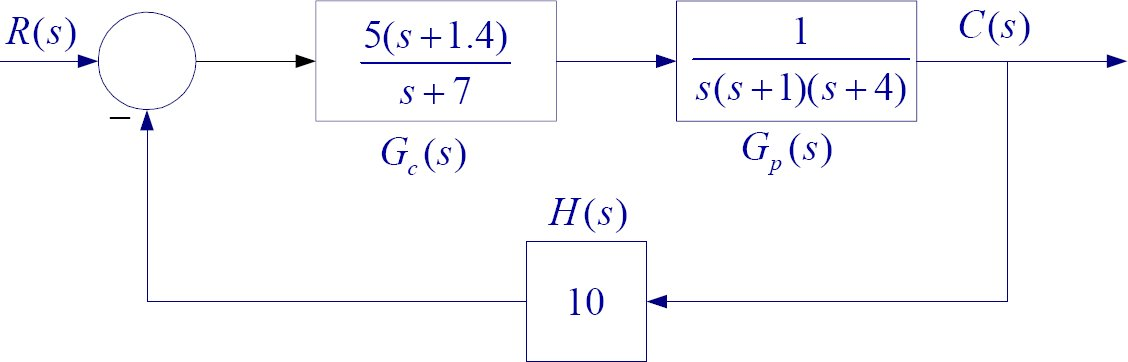
\includegraphics[width=.8\textwidth]{buildfeedback}
\caption{\footnotesize
        Block diagram in the frequency domain for the system in Example~\ref{ex.buildfeedback}.
        \label{fig.statespace.buildfeedback}
        }
\end{figure}

\begin{workex} \label{ex.buildfeedback}
Use the \verb=feedback= function to obtain the closed-loop transfer function and the \verb=tf2ss= function to obtain the closed-loop state space model of the system in Figure~\ref{fig.statespace.buildfeedback}.\\
\textit{Solution}:\\
The following commands should produce the desired result:
\begin{verbatim}
Gc = tf(5*[1 1.4],[1 7]);       % transfer function Gc
Gp = tf([1],[1 5 4 0]);         % transfer function Gp
H = 10;
G = series(Gc,Gp)               % connect Gc and Gp in cascade
T = feedback(G,H)               % close feedback loop
[num, den] = tfdata(T,'v')      % return num and den as row vectors
[A, B, C, D] = tf2ss(num,den)   % converts to state space model
\end{verbatim}

The transfer function should look like
\begin{verbatim}
                5 s + 7
     ---------------------------------
      s^4 12 s^3 + 39 s^2 + 78 s + 70
\end{verbatim}

And the matrices are
\begin{verbatim}
A =                     B =     C =                 D =
    -12 -39 -78 -70         1       0   0   5   7       0
    1   0   0   0           0
    0   1   0   0           0
    0   0   1   0           0
\end{verbatim}
\end{workex}

\section{MATLAB Functions for Modeling and Analysis}
Once a system is described by a certain model---be it in state space, by a transfer function, or otherwise---it is often important to perform some form of analysis on it.  How does it respond to different initial conditions?  Which inputs correspond to which outputs?  Is this thing stable or can we make it stable?  These are all questions we may ask of a system that comes presented to us as a ``black box.''
\par
The MATLAB Control System Toolbox contains the functions in Table~\ref{tab.statespace.ConSysToolTime} for analysis of time-domain response.

\begin{table}[bht]
\centering
\renewcommand{\arraystretch}{1.2}
\begin{tabular}{c|p{0.55\textwidth}}
    \textit{Command}& \multicolumn{1}{c}{\textit{Description}}\\ \hline \hline
    \verb=step=         &   Step response \\
    \verb=impulse=      &   Impulse response \\
    \verb=initial=      &   Response of a state space system to the given
                                initial state \\
    \verb=lsim=         &   Response to arbitrary inputs \\
    \verb=gensig=       &   Generates input signal for \verb=lsim= \\
    \verb=damp=         &   Natural frequency and damping of system poles \\
    \verb=ltiview=      &   Response analysis GUI (LTI System Viewer)
\end{tabular}
\caption{\footnotesize
        Time-domain system analysis functions
        \label{tab.statespace.ConSysToolTime}
        }
\end{table}
\par
Given a transfer function of a closed-loop control system, the function \verb=step(num,den)= produces the step response plot with the time vector automatically determined.  If the closed-loop system is defined in state space instead, we use \verb=step(A,B,C,D)= with or without subsequent optional arguments.  If output variables are specified for the \verb=step= function, say \verb=[y, t, x]=, then the output will be saved to \verb=y= for the time vector \verb=t=.  The array \verb=x= contains the trajectories of all of the state variables along the same time vector.  This syntax also applies to \verb=impulse=, \verb=initial=, and \verb=lsim=.

\vspace{6pt}
\begin{workex}  \label{ex.unitstep}
\begin{equation*}
    \frac{C(s)}{R(s)} =
        \frac{25(1+0.4s)}{ (1+0.16x)(x^2+6s+25)}
\end{equation*}
Obtain the unit step response of the system with the closed-loop transfer function above.  Also, use the \verb=damp= function to obtain the roots of the characteristic equation, the corresponding damping factors, and the natural frequencies.\\
\textit{Solution}:\\
The following code produces the response seen in Figure~\ref{fig.ex.unitstep}.
\begin{verbatim}
>> num = 25*[0.4 1];
>> den = conv([0.16 1], [1 6 25])   % Multiplies two polynomials.
>> T = tf(num,den)                  % Create TF object.
>> step(T), grid                    % Produces step response plot.
>> damp(T)                          % Produces data below:
        Eigenvalue              Damping         Freq. (rad/s)
        -3 + 4i                 6.00e-001           5.00
        -3 - 4i                 6.00e-001           5.00
        -6.25                   1.00e+000           6.25
>>
\end{verbatim}
The damping factors and natural frequencies are displayed in the right two columns.  The eigenvalues are the roots of the characteristic equation.
\end{workex}

\begin{figure}[thb]
\centering
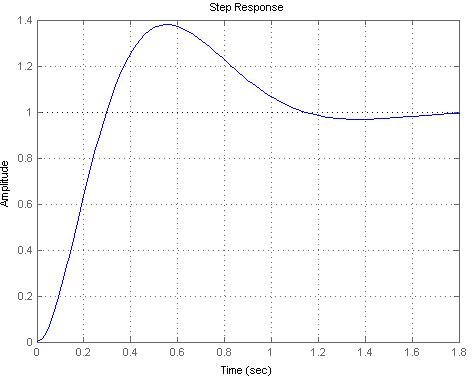
\includegraphics[width=.75\textwidth]{unitstep}
\caption{ \footnotesize
        Unit step response for system in Example \ref{ex.unitstep}
        \label{fig.ex.unitstep}
        }
\end{figure}

\begin{workex}  \label{ex.dompoles}
\begin{equation*}
    \frac{C(s)}{R(s)} = T(s) =
        \frac{750}{s^3 + 36s^2 + 205s + 750}
\end{equation*}
The closed-loop transfer function of a control system is described by the third-order transfer function $T(s)$.  Do the following:
\begin{enumerate}
\item
    Find the dominant poles of the system.
\item
    Find a reduced-order model.
\item
    Obtain the step response of the third-order system and the reduced-order system on the same figure plot.
\end{enumerate}
\textit{Solution}:\\
1. The poles are the roots of the denominator polynomial.  To find this, we use \verb=roots([1 36 205 750])=.  This gives us roots at $-30$ and $-3\pm4i$.  To determine dominance, we look at the time constants (negative inverse of real part) associated with these poles.  We see the pole at $-30$ has time constant $\tau_1 = 1/30$ where as the other two have time constant $\tau_2 = 1/3$.  The order of magnitude difference tells us that the poles at $3\pm4i$ are dominant. For more on time constants, see~\cite{dorf}, Section~2.5.\\
2. To reduce the model, we factor out the negligible pole and divide the numerator by its magnitude:
\begin{equation*}
    T(s) = \frac{750}{(s+30)(s^2 + 6s + 25)}
        \Rightarrow \tilde{T}(s) = \frac{25}{s^2 + 6s + 25}
\end{equation*}
\end{workex}\\
\begin{codex}
3. The following script produces the desired plot (Fig.\ \ref{fig.ex.dompoles}).
\begin{verbatim}
num1 = 750;
den1 = [1 36 205 750];
T = tf(num1,den1);              % Third-order system tf object.
num2 = 25;
den2 = [1 6 25];
Ttilde = tf(num2,den2);         % Reduced system tf object.
[y1 t] = step(T);               % Response and time vectors of T.
y2 = step(Ttilde,t);            % Response using the same time
                                    % vector of the reduced system.
plot(t,y1,'r-',t,y2,'b:')       % Put responses on the same plot.
grid;
xlabel('Time (s)');
ylabel('Displacement');
legend('Third-order','Reduced-order');
\end{verbatim}
\end{codex}

\begin{figure}[bht]
\centering
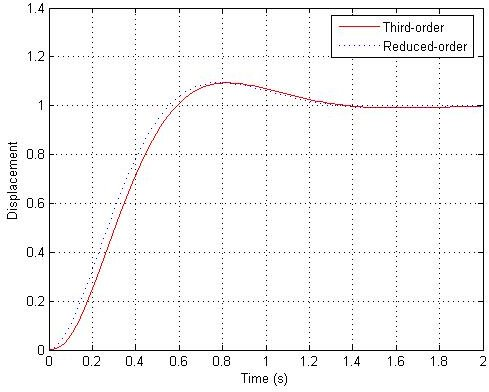
\includegraphics[width=.9\textwidth]{dompoles}
\caption{ \footnotesize
        Step responses of the original and reduced systems in Example~\ref{ex.dompoles}
        \label{fig.ex.dompoles}
        }
\end{figure}

\subsection{The LTI Viewer}
The Control System Toolbox LTI Viewer is a GUI (graphical user interface) that visually demonstrates the analysis of linear time-invariant systems.  We use the LTI Viewer to view and compare the response plots of several linear models at the same time.  We can also generate time- and frequency-domain response plots to inspect key response parameters such as rise time, maximum overshoot, and stability margins.  Using mouse-driven interactions, we can select input and output channels for multi-input, multi-output (MIMO) systems.  The LTI Viewer can display up to six different plot types simultaneously, including step and impulse responses, Bode, Nyquist, Nichols, sigma, and pole/zero diagrams.
\par
The command syntax is
\begin{verbatim}
ltiview('plot type',sys,extra)
\end{verbatim}
where \verb=sys= is the system object in question, and \verb='plot type'= is one of the following strings: \verb=step=, \verb=impulse=, \verb=initial=, \verb=lsim=, \verb=bode=, \verb=nyquist=, \verb=nichols=, or \verb=sigma=.  The optional argument \verb=extra= specifies the final time of the simulation.
\par
Once an LTI Viewer is open, a right-click of the mouse allows us to change the response type and obtain the system time-domain and frequency-domain specifications, such as those in Table~\ref{tab.ltiview}.

\begin{table}[bht]
\centering
\renewcommand{\arraystretch}{1.2}
\begin{tabular}{c|p{0.55\textwidth}}
    \textit{Menu Title}& \multicolumn{1}{c}{\textit{Description}}\\ \hline \hline
    Plot Type       &   Changes the plot type \\
    Systems         &   Selects any of the models loaded in the LTI Viewer \\
    Characteristics &   Displays key response characteristics and parameters\\
    Zoom            &   Zooms in and out of plot regions \\
    Grid            &   Adds grids to the plots \\
    Properties      &   Opens the Property Editor to customize plot attributes
\end{tabular}
\caption{\footnotesize
        LTI Viewer context-click menus
        \label{tab.ltiview}
        }
\end{table}

\begin{figure}[thb]
\centering
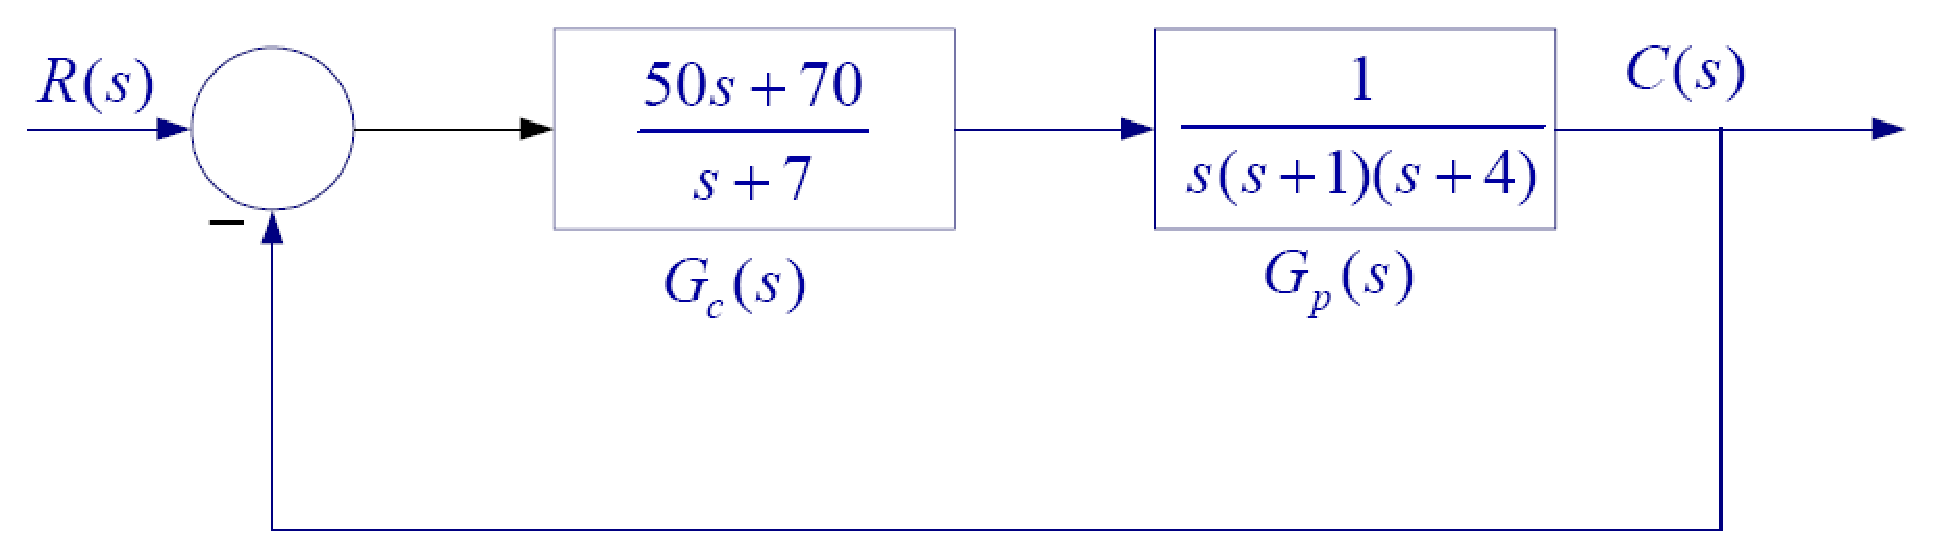
\includegraphics[width=.7\textwidth]{ltiviewexample}
\caption{ \footnotesize
        Block diagram for Example~\ref{ex.ltiview}
        \label{fig.ex.ltiview}
        }
\end{figure}

\begin{workex}  \label{ex.ltiview}
Use the LTI Viewer to obtain the step response and the time-domain specifications for the control system shown in Fig.\ \ref{fig.ex.ltiview}.\\
\textit{Solution}:\\
We use the following commands to generate the response plot in Figure~\ref{fig.ex.ltiviewstep}.
\begin{verbatim}
>> Gc = tf([50 70],[1 7]);      % Transfer function Gc.
>> Gp = tf([1],conv([1 1 0],[1 4]));    % Transfer function Gp,
                                % with expanded denominator.
>> H = 1;                       % Unity feedback.
>> G = series(Gc,Gp);           % Connect Gc and Gp in cascade.
>> T = feedback(G,H)            % Close unity feedback loop.

Transfer function:
            50 s + 70
---------------------------------
s^4 + 12 s^3 + 39 s^2 + 78 s + 70

>> ltiview('step',T)
>>
\end{verbatim}
\end{workex}

\begin{figure}[bht]
\centering
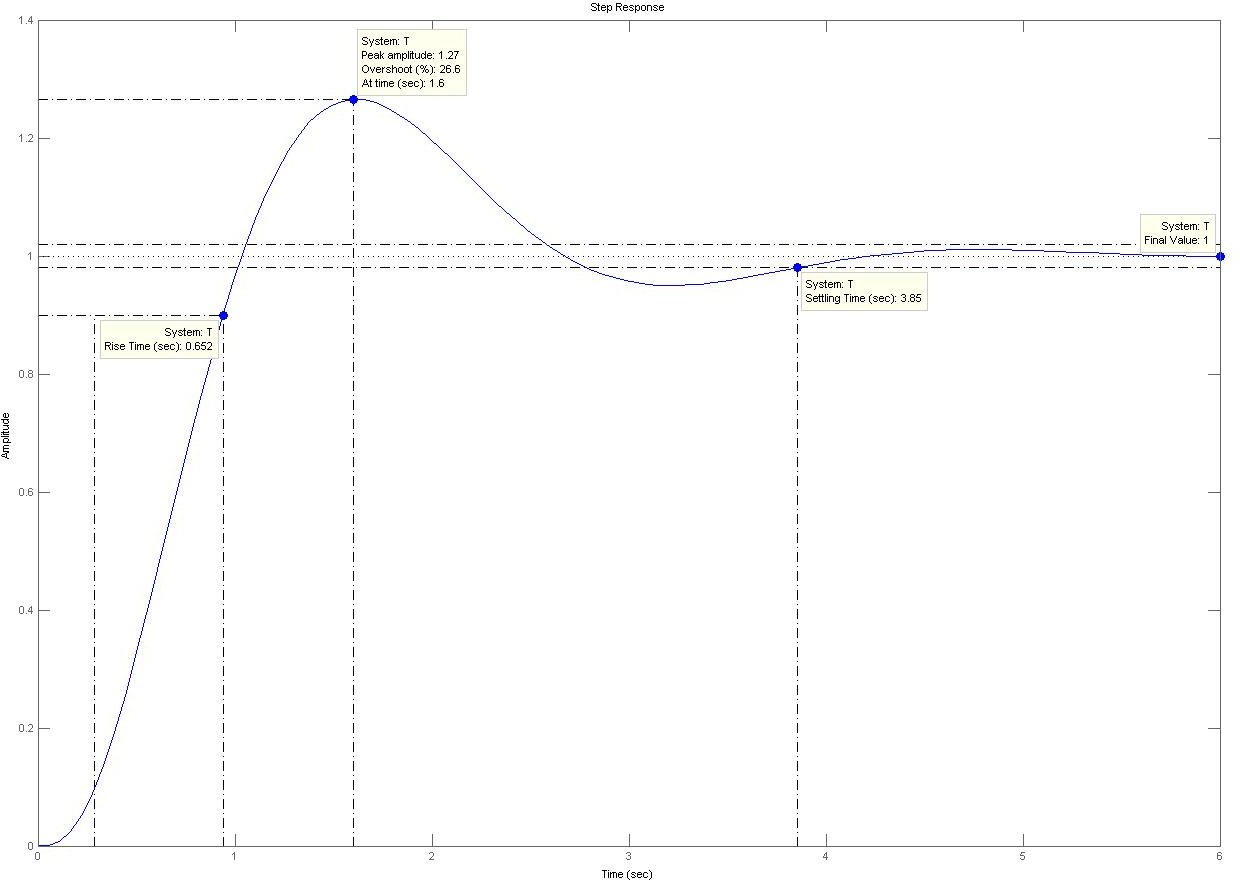
\includegraphics[width=.9\textwidth]{ltiviewstep}
\caption{ \footnotesize
        Step response with metadata tags for Example~\ref{ex.ltiview}
        \label{fig.ex.ltiviewstep}
        }
\end{figure}
\par
For time-domain analysis, it is often much easier to use the LTI Viewer because it is possible to obtain many system parameters with a simple right-click of the mouse.  In addition, it allows us to select from a myriad of responses and data projections via the Plot Type.

\subsection{Numerical Solutions of Differential Equations}
There are many powerful techniques in MATLAB for the numerical solution of nonlinear equations.  A popular technique is the Runge-Kutta method, which is based on formulas derived by using an approximation to replace the truncated Taylor series expansion.  The interested reader should see \cite{butcher} or an equivalent text on numerical methods.
\par
MATLAB provides several powerful functions for the numerical solution of differential equations: See Table~\ref{tab.odesolvers}.  Two of the functions employing the Runge-Kutta-Fehlberg methods are \verb=ode23= and \verb=ode45=; they are based on the Fehlberg second- and third-order pair of formulas for medium accuracy and the fourth- and fifth-order pair for higher accuracy.

\begin{table}[bht]
\centering
\renewcommand{\arraystretch}{1.2}
\begin{tabular}{c|p{0.55\textwidth}}
    \textit{Command}& \multicolumn{1}{c}{\textit{Description}}\\ \hline \hline
    \verb=ode23=        &   Solve non-stiff differential equations,
                                low order method \\
    \verb=ode45=        &   Solve non-stiff differential equations,
                                medium order method
\end{tabular}
\caption{\footnotesize
        Numerical solvers for ordinary differential equations
        \label{tab.odesolvers}
        }
\end{table}
\par
The $n^{th}$-order differential equation must be transformed first into $n$ first-order differential equations and must be placed in an m-file that returns the derivative of the state equations.  This file's name is represented as the string \verb='xprime'= in the general syntax below:
\begin{verbatim}
[t, x] = ode23('xprime',tspan,x0,option)
\end{verbatim}
Also, \verb=tspan= is a vector of times covering the interval of integration, and \verb=x0= is a column vector of initial state conditions.  Commonly used options are scalar relative error tolerance (\verb#RelTol = 1e-3# by default) and vector absolute error tolerances (all elements of \verb#AbsTol = 1e-6# by default).

\begin{workex}  \label{ex.ode23}
\begin{equation*}
    \frac{d^2\theta}{dt^2} + \frac{B}{m} \frac{d\theta}{dt} +
        \frac{g}{l} \sin \theta = 0
\end{equation*}
The above equation describes the motion of the simple pendulum derived in Lab Session \ref{ch.ModSim}, Case Study \ref{cs.simplepend}.  Using the MATLAB function \verb=ode23=, obtain the numerical solution for the following values:
\begin{itemize}
    \item $m = 0.5$kg and $l = 0.613$m
    \item $B = 0.05$kg-s/m and $g = 9.81$m/s/s
    \item $\theta(t=0) = \dot{\theta}(t=0) = 0$
\end{itemize}

\end{workex}


\begin{thebibliography}{9}
    \bibitem{dorf} Richard C. Dorf and Robert H. Bishop.  Modern Control Systems, 11th edition.  Prentice Hall, Upper Saddle River, NJ.  2008.
    \bibitem{firsted} EE351L Laboratory Manual, 1st edition.
    \bibitem{butcher} John C. Butcher.  Numerical Methods for Ordinary Differential Equations, 2nd edition.  John Wiley.  2003.
\end{thebibliography}
